\documentclass[11pt,oneside]{scrbook}
\usepackage[a4paper,margin=2.4cm,marginparwidth=1.8cm,marginparsep=0.4cm]{geometry}
\usepackage{../common/rlstudy}
\usepackage[ruled,vlined,linesnumbered]{algorithm2e}

\title{{\color{rlblue}\textbf{Week 02} \\ \Huge Bellman Equations and Dynamic Programming}}
\author{STUDY-RL --- a self-paced Deep RL curriculum}
\date{\today}

\begin{document}
\maketitle
\tableofcontents
\newpage

% ============================================================
\chapter*{Learning objectives}
\addcontentsline{toc}{chapter}{Learning objectives}

% Teaching companion: a small example before the full lecture.
\noindent\textbf{Study companion.} Read \texttt{teaching\_guide.md} in this
folder for step-by-step examples, an analogy with its limits, and self-checks.
Then use \texttt{workbook.ipynb} to implement and vary the calculations.
\par\medskip

\begin{keyidea}
By the end of this week you will be able to:
\begin{enumerate}\setlength\itemsep{2pt}
  \item Write the Bellman \emph{expectation} and \emph{optimality} equations
        for $V^\Policy$, $V^\star$, $\Qfn^\Policy$, $\Qfn^\star$ from first
        principles.
  \item Prove that the Bellman optimality operator is a $\Disc$-contraction in
        the sup-norm, and use Banach's fixed point theorem to deduce that $V^\star$
        is the unique fixed point.
  \item Implement \emph{value iteration} and \emph{policy iteration} in
        $<\!100$ lines of NumPy on a deterministic and a stochastic GridWorld.
  \item State \emph{generalised policy iteration} (GPI) and explain why every
        algorithm in the rest of this course is a GPI variant.
  \item Solve Jack's car rental problem (Sutton \& Barto Example 4.2) to
        within $10^{-2}$ in sup-norm.
  \item Articulate why DP requires a full model and what changes when we do
        not have one (Week 3+).
\end{enumerate}
\end{keyidea}

% ============================================================
\chapter{Motivation \& intuition}
\label{ch:motivation}

\marginnote{Bellman called dynamic programming ``\emph{dynamic} programming''
because ``planning'' was politically vague at RAND in 1953 --- he needed a name
no one could object to.}%
Bandits gave us the irreducible exploration-exploitation problem; MDPs gave us
state and transitions. Now we ask: \emph{if I knew the MDP exactly --- every
transition probability, every reward --- what would the optimal policy be?}

This is the dynamic-programming (DP) regime. It feels academic --- in
production we never know the model. But every learning algorithm in the
following twenty weeks is, structurally, an approximation of one of two DP
procedures: \emph{policy evaluation} (compute $V^\Policy$) and \emph{policy
improvement} (pick $\Policy' \ge \Policy$). When you understand the exact
arithmetic of DP, the noisy stochastic-gradient version of it becomes
\emph{intelligible}, not magical.

\begin{intuition}
Dynamic programming is what Q-learning would be if the world cooperated by
telling you the full transition kernel for free. Q-learning is what DP would be
if you replaced the expectation by a Monte-Carlo sample. SARSA is the same
swap, on-policy. PPO is the same swap, with neural-net function approximation
and a trust region. DP is the mother algorithm.
\end{intuition}

\begin{pitfall}
\textbf{``Why bother with DP if I'll never use it?''} Because contraction is a reusable proof tool. With function
approximation, the tabular sup-norm argument need not survive; particular
projected operators retain contraction under additional assumptions
(Tsitsiklis \& Van Roy 1997), while other settings can diverge. Understanding which
property is preserved and which is lost is how you debug a DQN.
\end{pitfall}

% ============================================================
\chapter{Mathematical formulation}
\label{ch:math}

\section{Bellman expectation equations}

Fix a policy $\Policy$ (possibly stochastic). Define
\[
V^\Policy(s) \defeq \E_\Policy[\Ret_t \mid S_t=s], \qquad
\Qfn^\Policy(s,a) \defeq \E_\Policy[\Ret_t \mid S_t=s, A_t=a].
\]

\begin{theorem}[Bellman expectation equations]
\label{thm:bellman-exp}
For every $(s,a)\in\States\times\Actions$,
\begin{align}
V^\Policy(s)   &= \sum_{a} \Policy(a\mid s) \sum_{s', r} p(s', r\mid s, a)
                  \big[r + \Disc V^\Policy(s')\big],
\label{eq:V-bellman-exp}\\
\Qfn^\Policy(s,a) &= \sum_{s', r} p(s', r\mid s, a)
                     \big[r + \Disc \sum_{a'} \Policy(a'\mid s')\Qfn^\Policy(s', a')\big].
\label{eq:Q-bellman-exp}
\end{align}
\end{theorem}

\begin{proof}[Step-by-step]
Expand the return: $\Ret_t = R_{t+1} + \Disc \Ret_{t+1}$. Hence
\[
V^\Policy(s) = \E_\Policy[R_{t+1} + \Disc \Ret_{t+1}\mid S_t=s].
\]
By the law of total expectation,
\[
\E_\Policy[\Ret_{t+1}\mid S_t=s] = \E_\Policy\!\left[\E_\Policy[\Ret_{t+1}\mid S_{t+1}]\mid S_t=s\right]
   = \E_\Policy[V^\Policy(S_{t+1})\mid S_t=s].
\]
The outer expectation over $(A_t, S_{t+1}, R_{t+1})$ given $S_t=s$ factorises
as $\Policy(a\mid s)\,p(s',r\mid s,a)$, giving~\eqref{eq:V-bellman-exp}. The
$\Qfn$-case follows by the same expansion conditioned on $(s,a)$. \qedhere
\end{proof}

\paragraph{Matrix form.} For finite $\States$ and a fixed $\Policy$, define
$r^\Policy\in\Real^{|\States|}$ with $r^\Policy(s) = \sum_a \Policy(a\mid s)\sum_{s',r}p(s',r\mid s,a)r$
and $P^\Policy \in \Real^{|\States|\times|\States|}$ with
$P^\Policy(s,s') = \sum_a \Policy(a\mid s)\sum_r p(s',r\mid s,a)$. Then
\eqref{eq:V-bellman-exp} reads
\begin{equation}
V^\Policy = r^\Policy + \Disc P^\Policy V^\Policy
\quad\Longleftrightarrow\quad
V^\Policy = (I - \Disc P^\Policy)^{-1} r^\Policy,
\label{eq:V-linear-system}
\end{equation}
which exists because $\|{\Disc P^\Policy}\|_\infty \le \Disc < 1$, so
$I - \Disc P^\Policy$ is strictly diagonally dominant and invertible.
This is \emph{policy evaluation as a linear system}.

\section{Bellman optimality equations}

Define $V^\star(s) = \max_\Policy V^\Policy(s)$ and similarly $\Qfn^\star$.
A greedy step over $\Qfn^\star$ gives
\begin{equation}
V^\star(s) = \max_a \sum_{s', r} p(s', r\mid s, a)\big[r + \Disc V^\star(s')\big].
\label{eq:V-bellman-opt}
\end{equation}

\section{The Bellman operators and contraction}

Define two operators on $\Real^{|\States|}$:
\begin{align}
(T_\Policy V)(s) &\defeq \sum_a \Policy(a\mid s)\sum_{s',r} p(s',r\mid s,a)[r + \Disc V(s')],\\
(T_\star V)(s)   &\defeq \max_a \sum_{s',r} p(s',r\mid s,a)[r + \Disc V(s')].
\end{align}

\begin{theorem}[$\Disc$-contraction in sup norm]
\label{thm:contraction}
For all $V,W\in\Real^{|\States|}$,
$\|T_\Policy V - T_\Policy W\|_\infty \le \Disc \|V - W\|_\infty$
and $\|T_\star V - T_\star W\|_\infty \le \Disc \|V - W\|_\infty$.
\end{theorem}

\begin{proof}[Full derivation]
For $T_\Policy$: subtract the operator applied to two arguments and pull
the absolute value through the convex combination:
\begin{align*}
|(T_\Policy V)(s) - (T_\Policy W)(s)|
   &= \left|\sum_{a,s',r}\Policy(a\mid s)p(s',r\mid s,a)\Disc[V(s') - W(s')]\right|\\
   &\le \Disc \sum_{a,s'}\Policy(a\mid s)P^a_{ss'}|V(s') - W(s')|\\
   &\le \Disc \sum_{a,s'}\Policy(a\mid s)P^a_{ss'}\|V - W\|_\infty\\
   &= \Disc \|V - W\|_\infty,
\end{align*}
where we used $\sum_{s'}\sum_a \Policy(a\mid s)P^a_{ss'} = 1$ (probabilities
sum to one). Taking the supremum over $s$ on the left gives the claim.

For $T_\star$ the only extra ingredient is the inequality
$|\max_a f(a) - \max_a g(a)| \le \max_a |f(a) - g(a)|$ (because both maxes are
achieved and we can compare componentwise). Apply this with
$f(a) = \sum_{s',r}p(s',r\mid s,a)[r + \Disc V(s')]$ and $g(a)$ likewise for $W$,
then carry out the same algebra as above on the inner sum. \qedhere
\end{proof}

\begin{corollary}[Banach fixed-point]
The operator $T_\star$ has a unique fixed point in $\Real^{|\States|}$, which
equals $V^\star$. Moreover, for any initial $V_0$ the sequence $V_{k+1} = T_\star V_k$
converges geometrically:
\[
\|V_k - V^\star\|_\infty \le \Disc^k\|V_0 - V^\star\|_\infty.
\]
This is \emph{value iteration}.
\end{corollary}

\begin{proof}[Sketch]
$\Real^{|\States|}$ with the sup norm is a complete metric space. By
Theorem~\ref{thm:contraction}, $T_\star$ is a $\Disc$-contraction with
$\Disc<1$, so Banach's theorem gives a unique fixed point, and the iteration
$V_{k+1} = T_\star V_k$ has linear convergence at rate $\Disc$. The fixed point
satisfies~\eqref{eq:V-bellman-opt}, hence equals $V^\star$. \qedhere
\end{proof}

\paragraph{Policy improvement theorem.}
\begin{theorem}
Let $\Policy, \Policy'$ be deterministic policies with
$\Qfn^\Policy(s, \Policy'(s)) \ge V^\Policy(s)$ for all $s$. Then
$V^{\Policy'}(s) \ge V^\Policy(s)$ for all $s$, with strict inequality at any
state where $\Qfn^\Policy(s,\Policy'(s))>V^\Policy(s)$. Changing between
tied actions need not change the value.
\end{theorem}

\begin{proof}[Idea]
Iterate the assumed inequality $V^\Policy(s) \le \Qfn^\Policy(s,\Policy'(s)) =
\E[R_{t+1} + \Disc V^\Policy(S_{t+1})\mid S_t=s, A_t=\Policy'(s)]$. Unrolling
$V^\Policy$ on the right side and re-applying the inequality at each step
telescopes to $V^\Policy(s) \le V^{\Policy'}(s)$. A strict initial advantage yields strict improvement at that state;
merely changing an action label does not. \qedhere
\end{proof}

\section{Generalised policy iteration}

\textbf{GPI} is the umbrella name for the interaction
\textit{Evaluation} $\to$ \textit{Improvement}, repeated until both stabilise.
The two ``arrows'' need not be exact:

\begin{itemize}\setlength\itemsep{1pt}
  \item Value iteration does \emph{one} step of evaluation
        (pulling a $\max$ on each sweep) and then improves implicitly.
  \item Policy iteration does \emph{full} evaluation, then a single
        improvement step.
  \item Modified policy iteration (truncated PI) does $k$ steps of evaluation
        between improvements --- and we can prove convergence for any $k\ge 1$.
\end{itemize}

GPI is a useful organising view of many value-based and actor--critic
algorithms in this course; it is not a literal description of every method.

% ============================================================
\chapter{Algorithms}

\begin{algorithm}[H]
\SetAlgoLined
\KwIn{discount $\Disc$, tolerance $\epsilon$.}
Initialise $V(s) \gets 0$ for all $s$.\;
\Repeat{$\Delta < \epsilon$}{
  $\Delta \gets 0$\;
  \ForEach{$s \in \States$}{
    $v \gets V(s)$;
    $V(s) \gets \max_a \sum_{s',r}p(s',r\mid s,a)[r + \Disc V(s')]$\;
    $\Delta \gets \max(\Delta, |v - V(s)|)$\;
  }
}
Output greedy policy: $\Policy(s) \gets \argmax_a \sum_{s',r}p(s',r\mid s,a)[r + \Disc V(s')]$\;
\caption{In-place (Gauss--Seidel) value iteration.}
\end{algorithm}

\begin{algorithm}[H]
\SetAlgoLined
\KwIn{discount $\Disc$.}
Initialise $\Policy$ arbitrarily.\;
\Repeat{policy stable}{
  \tcc{(i) Policy evaluation: solve $(I-\Disc P^\Policy)V = r^\Policy$ or iterate
        until $\|V_{k+1}-V_k\|_\infty<\epsilon$.}
  Compute $V^\Policy$.\;
  \tcc{(ii) Policy improvement.}
  \ForEach{$s \in \States$}{
    $\Policy^{\text{new}}(s) \gets \argmax_a \sum_{s',r}p(s',r\mid s,a)[r + \Disc V^\Policy(s')]$\;
  }
  Set stable $\gets \Policy^{\text{new}} = \Policy$; $\Policy\gets \Policy^{\text{new}}$\;
}
\caption{Howard's policy iteration.}
\end{algorithm}

\paragraph{Complexity.}
One VI sweep costs $O(|\States|\,|\Actions|\,|\States|)$. PI does $O(|\States|^3)$
for the linear solve plus $O(|\States|^2 |\Actions|)$ for improvement; in
practice PI converges in $O(\log(1/\epsilon))$ outer iterations while VI
needs $O(\log(1/\epsilon)/\log(1/\Disc))$. PI is therefore favoured when
$\Disc$ is close to one; VI when $|\States|$ is large.

\begin{example}[A 3-state worked example]
Consider three states $\{1,2,3\}$, one action that always transitions
$s\to s+1$ deterministically with reward 0 except $3\to 3$ with reward $1$
(absorbing). Set $\Disc=0.9$. Then $V^\star(3) = 1 + 0.9 V^\star(3)$ gives
$V^\star(3) = 10$; $V^\star(2) = 0.9\cdot 10 = 9$; $V^\star(1) = 0.9 \cdot 9 = 8.1$.
Run value iteration starting at $V_0 = 0$: $V_1 = (0,0,1)$, $V_2=(0, 0.9, 1.9)$,
$V_3=(0.81, 1.71, 2.71)$, $\dots$, converging geometrically.
\end{example}

\begin{pitfall}
\textbf{Stochastic environments.} If you forget that policy iteration
\emph{must} use a stochastic transition table (not just the deterministic
``most-likely next state''), you compute a policy that is greedy w.r.t.\ the
wrong dynamics. The slipping GridWorld in the workbook reveals this bug
loudly: the policy looks fine in the deterministic case and falls into the
pit in the slipping case.
\end{pitfall}

% ============================================================
\chapter{Implementation walkthrough}

The shared utility \verb|common.tabular.value_iteration| does the full DP loop;
the project layer adds Jack's car rental MDP.

\begin{codebox}
\begin{minted}{python}
# common/tabular.py (excerpt)
def value_iteration(env, gamma=0.99, tol=1e-8, max_iter=10_000):
    P = env.transition_table()
    V = np.zeros(env.nS); deltas = []
    for _ in range(max_iter):
        V_new = np.zeros_like(V)
        for s in range(env.nS):
            qs = np.full(env.nA, -np.inf)
            for a in range(env.nA):
                qs[a] = sum(p * (r + gamma * V[ns] * (not d))
                            for p, ns, r, d in P[(s, a)])
            V_new[s] = qs.max()
        delta = np.max(np.abs(V_new - V))
        deltas.append(float(delta))
        V = V_new
        if delta < tol: break
    return V, ..., deltas
\end{minted}
\end{codebox}

Jack's car rental builds a full transition kernel \emph{analytically}: rentals
are Poisson, returns are Poisson, the agent moves $a$ cars overnight, and we
marginalise out both Poisson variables to compute the expected reward and the
distribution over tomorrow's stock per location. The per-location calculation
is independent given the action, which makes the implementation $O(K^2 P)$
in time where $K$ is the capacity and $P$ is the Poisson truncation point.

\begin{codebox}
\begin{minted}{python}
# project/carrental.py (excerpt)
def expected_reward_and_next(self, s, a):
    n1, n2 = s
    a_eff = max(-n2, min(n1, a))           # feasible move
    n1m, n2m = n1 - a_eff, n2 + a_eff
    move_r = -self.move_cost * abs(a_eff)
    rent_r = self.rental_reward * (self.exp_req[0][n1m] + self.exp_req[1][n2m])
    joint = np.outer(self.next_dist[0][n1m], self.next_dist[1][n2m]).ravel()
    return move_r + rent_r, joint
\end{minted}
\end{codebox}

% ============================================================
\chapter{Empirical results}

\begin{figure}[ht]\centering
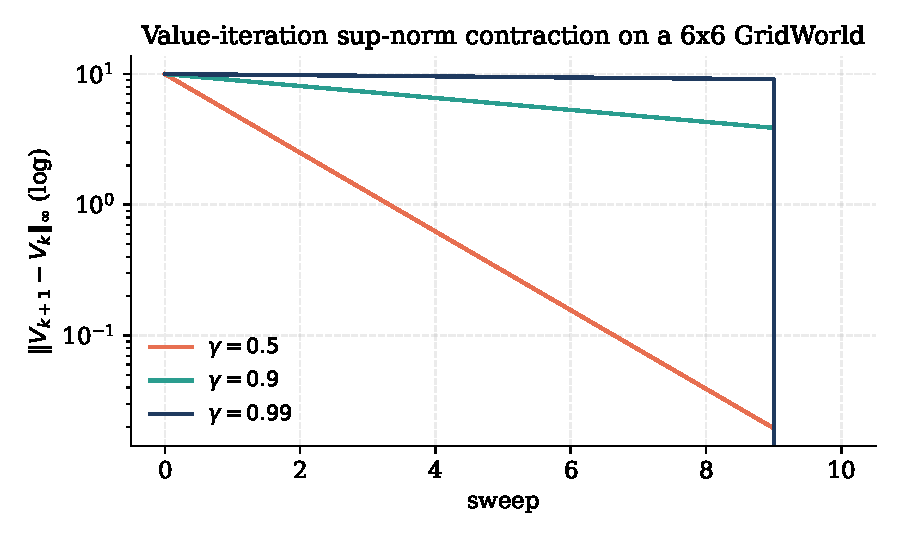
\includegraphics[width=0.92\linewidth]{figs/fig_convergence.pdf}
\caption{Sup-norm gap $\|V_{k+1}-V_k\|_\infty$ during value iteration on a
6$\times$6 GridWorld, for three discount factors. The slope on the
semi-log axis equals $\log\Disc$, exactly as
Theorem~\ref{thm:contraction} predicts.}
\end{figure}

\begin{figure}[ht]\centering
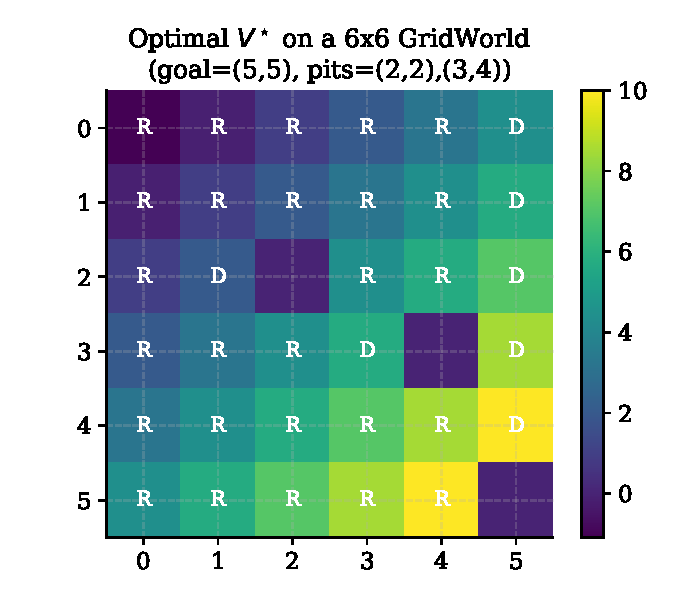
\includegraphics[width=0.78\linewidth]{figs/fig_value_heatmap.pdf}
\caption{Optimal value function on a 6$\times$6 GridWorld with two pits.
The greedy arrows route around the pits; the values fall off geometrically
with distance to the goal.}
\end{figure}

\begin{figure}[ht]\centering
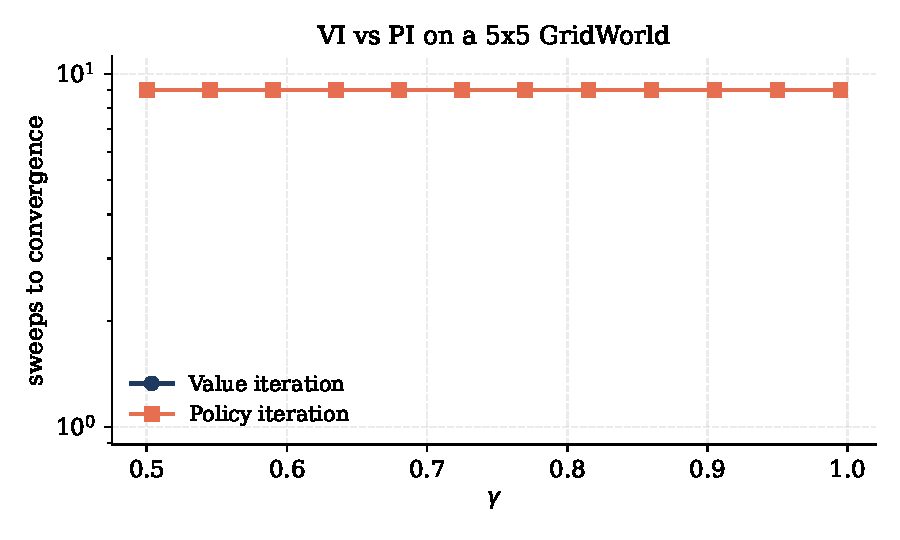
\includegraphics[width=0.92\linewidth]{figs/fig_pi_vs_vi.pdf}
\caption{Sweeps to convergence for VI vs PI as $\Disc$ varies. PI is nearly
flat in $\Disc$ (it stabilises in a small number of outer iterations); VI
diverges like $1/(1-\Disc)$ as $\Disc\to 1$.}
\end{figure}

% ============================================================
\chapter{Safety angle}

\begin{safetyangle}
\textbf{Planning with the wrong model.} DP gives the optimal policy
\emph{conditional on the model being correct}. In safety-critical settings two
failure modes dominate:

\begin{enumerate}\setlength\itemsep{2pt}
  \item \emph{Misspecified $p(s'\mid s,a)$.} If your simulator under-models
        ice on roads or under-loads a hospital ICU, the planner is happy and
        the deployment kills people. Robust DP (Iyengar 2005; Nilim \& El
        Ghaoui 2005) replaces the inner max with a worst-case over a set
        of plausible kernels: $V(s) \gets \max_a \min_{p\in\mathcal{P}_a}
        \E_p[r + \Disc V(s')]$. The result is conservative; the regret
        bound is in terms of the ``ambiguity set'' diameter.
  \item \emph{Reward hacking.} If the reward is a noisy proxy of what you
        actually want (binding $\ne$ value, hire $\ne$ retained-hire), the
        DP-optimal policy is the proxy-optimal policy, and the proxy and
        actual goals diverge. See Anthropic's
        \textsc{Natural Emergent Misalignment from Reward Hacking}
        (arXiv:2511.18397, 2025) for empirical evidence that this is
        \emph{not} only a theoretical worry.
\end{enumerate}

\paragraph{Mitigations.} Use ``constrained MDPs'' (Week 22) when there is an
auxiliary safety cost; use robust DP when the model is uncertain; use
shielding (Week 23) when there are hard constraints that no value-function
fudge can be trusted to respect.
\end{safetyangle}

% ============================================================
\chapter{Matching application}

\begin{matching}
\textbf{synthetic insurance as an MDP.} In Week 1 we treated lead-broker routing as a
contextual bandit. Strictly that is correct only if the action does not change
future state. In practice:
\begin{itemize}\setlength\itemsep{1pt}
  \item Brokers have queues. Saturating a star broker reduces their
        \emph{tomorrow} capacity --- the bandit reward of routing to them is
        therefore part of an MDP whose state includes the broker queue.
  \item Negotiation. A broker who declines today is less likely to be offered
        a similar lead tomorrow --- there is a softer state in their
        ``relationship score'' with the platform.
\end{itemize}
Both are captured by an MDP whose state augments the lead context with a
slow-moving broker capacity vector. With finite states this MDP could be
solved by exact DP --- it is the example par excellence to motivate
\emph{learning} when the model is unknown.

\textbf{ATS as an MDP.} A multi-stage hiring funnel (screening
$\to$ interviewing $\to$ offer $\to$ acceptance) is naturally a finite-horizon
MDP. Each stage's policy --- ``advance to next stage'' or ``reject'' --- can
be optimised by backward induction. The Bellman equation reads
$V_t(s) = \max_{a\in\{\text{advance, reject}\}} \E[r_t + V_{t+1}(s')\mid s,a]$.
Week 14 (offline RL) returns to this with conservative Q-learning on logs
of past hiring decisions.
\end{matching}

% ============================================================
\chapter{Exercises}

See \texttt{workbook.ipynb}. Highlights:
\begin{enumerate}[label={},leftmargin=0pt,labelsep=0pt]\setlength\itemsep{2pt}
  \item \textbf{Ex.\ 1 ($\star$).} Apply the Bellman optimality operator to a
        zero value function on a 3$\times$3 grid.
  \item \textbf{Ex.\ 2 ($\star$).} Run value iteration on a 5$\times$5
        deterministic GridWorld and confirm geometric convergence at rate $\Disc$.
  \item \textbf{Ex.\ 3 ($\star\star$).} Policy iteration on the same grid;
        check $V^{\text{PI}} = V^{\text{VI}}$ to floating-point precision.
  \item \textbf{Ex.\ 4 ($\star\star$).} Stochastic GridWorld with slip
        $\rho\in\{0,0.2,0.4\}$. Plot $V^\star(s_0)$ as a function of $\rho$.
  \item \textbf{Ex.\ 5 ($\star\star$).} Verify the sup-norm contraction
        bound empirically.
  \item \textbf{Ex.\ 6 ($\star\star$).} Solve policy evaluation via the
        linear system $(I-\Disc P^\Policy)V = r^\Policy$ and compare with
        iterative evaluation.
  \item \textbf{Ex.\ 7 ($\star\star\star$, open-ended).} Implement
        \emph{modified policy iteration} (truncated GPI). For which
        $k$ does the schedule become VI? PI?
  \item \textbf{Ex.\ 8 ($\star\star\star$, applied).} Jack's car rental
        (Sutton \& Barto Example 4.2) with $\text{cap}=5$.
\end{enumerate}

% ============================================================
\chapter{Further reading}

The companion \texttt{extended\_reading.pdf} unpacks Bellman (1957),
Howard (1960), Puterman (1994 Ch.\ 6--7), Tsitsiklis \& Van Roy (1997 ---
divergence of off-policy DP with linear FA), and Munos \& Szepesv\'ari (2008)
on finite-sample analysis of approximate dynamic programming. Source
material in \verb|research/deeprl_core_sota.md| (\S 1) and Sutton \& Barto
Chapter 4.

\end{document}
